
%%%%%%%%%%%%%%%%%%%%%%% file typeinst.tex %%%%%%%%%%%%%%%%%%%%%%%%%
%
% This is the LaTeX source for the instructions to authors using
% the LaTeX document class 'llncs.cls' for contributions to
% the Lecture Notes in Computer Sciences series.
% http://www.springer.com/lncs       Springer Heidelberg 2006/05/04
%
% It may be used as a template for your own input - copy it
% to a new file with a new name and use it as the basis
% for your article.
%
% NB: the document class 'llncs' has its own and detailed documentation, see
% ftp://ftp.springer.de/data/pubftp/pub/tex/latex/llncs/latex2e/llncsdoc.pdf
%
%%%%%%%%%%%%%%%%%%%%%%%%%%%%%%%%%%%%%%%%%%%%%%%%%%%%%%%%%%%%%%%%%%%


\documentclass[runningheads,a4paper]{llncs}

\usepackage{amssymb}
\setcounter{tocdepth}{3}
\usepackage{graphicx}

\usepackage[linesnumbered,ruled,vlined]{algorithm2e}

\usepackage{url}
\urldef{\mailsa}\path|{alfred.hofmann, ursula.barth, ingrid.haas, frank.holzwarth,|
\urldef{\mailsb}\path|anna.kramer, leonie.kunz, christine.reiss, nicole.sator,|
\urldef{\mailsc}\path|erika.siebert-cole, peter.strasser, lncs}@springer.com|    
\newcommand{\keywords}[1]{\par\addvspace\baselineskip
\noindent\keywordname\enspace\ignorespaces#1}

\usepackage{tikz}
\usepackage{aeguill}
\usepackage{tikzscale}
\usepackage{filecontents} 


\begin{document}

\mainmatter  % start of an individual contribution

% first the title is needed
\title{DataONE RunManager: Capturing Provenance of R and Matlab Scripts}

% a short form should be given in case it is too long for the running head
\titlerunning{Lecture Notes in Computer Science: Authors' Instructions}

% the name(s) of the author(s) follow(s) next
%
% NB: Chinese authors should write their first names(s) in front of
% their surnames. This ensures that the names appear correctly in
% the running heads and the author index.
%
\author{
TBD
% Alfred Hofmann%
% \thanks{Please note that the LNCS Editorial assumes that all authors have used
% the western naming convention, with given names preceding surnames. This determines
% the structure of the names in the running heads and the author index.}%
% \and Ursula Barth\and Ingrid Haas\and Frank Holzwarth\and\\
% Anna Kramer\and Leonie Kunz\and Christine Rei\ss\and\\
% Nicole Sator\and Erika Siebert-Cole\and Peter Stra\ss er}
%
%\authorrunning{Lecture Notes in Computer Science: Authors' Instructions}
% (feature abused for this document to repeat the title also on left hand pages)

% the affiliations are given next; don't give your e-mail address
% unless you accept that it will be published
\institute{TBD
% Springer-Verlag, Computer Science Editorial,\\
% Tiergartenstr. 17, 69121 Heidelberg, Germany\\
% \mailsa\\
% \mailsb\\
% \mailsc\\
% \url{http://www.springer.com/lncs}
}

%
% NB: a more complex sample for affiliations and the mapping to the
% corresponding authors can be found in the file "llncs.dem"
% (search for the string "\mainmatter" where a contribution starts).
% "llncs.dem" accompanies the document class "llncs.cls".
%

\toctitle{Lecture Notes in Computer Science}
\tocauthor{Authors' Instructions}
\maketitle


\begin{abstract}
The abstract should summarize the contents of the paper and should
contain at least 70 and at most 150 words. It should be written using the
\emph{abstract} environment.
\keywords{We would like to encourage you to list your keywords within
the abstract section}
\end{abstract}


\section{Introduction}

Scientific workflow provenance tracking is well recognized as a valuable approach in computational science. The term \emph{provenance} originally is used in the art world to establish the authentication of a work of art. Provenance has been used in other fields as well. For example, provenance in the field of the scientific workflow refers to having knowledge of all the steps involved in producing a scientific result.  Such information can help scientists to better understand their work. Additionally, scientists can document their experiments and share experimental data and computational steps with other researchers.  These activities can be called \emph{reproducible research}.

Scientific workflow systems support two aspects of provenance information: \emph{prospective} and \emph{retrospective} provenance. Prospective provenance presents a workflow as a directed graph with data and planned computational steps, while retrospective provenance captures the context of a script execution. 

There are many workflow management systems such as Taverna, Kepler, Galaxy that can transparently track, query, and visualize the scientific provenance information such as intermediate results, workflow steps, and parameter settings.  But many scientists prefer to use programming languages (such as R, Matlab, Python) for scientific computing work without using workflow management systems. For this end, several provenance tracking systems (such as Sumatra \cite{sumatra} \cite{sumatra-impl}, noWorkflow \cite{noworkflow} and RDataTracker \cite{rdatatracker}) have been implemented to assist scientists to capture and analyze the provenance traces of script execution. 

The existing work for capturing provenance for scientific workflow is presented in Section \ref{related-work}. We have developed a DataONE \emph{RunManager} for capturing the prospective and the retrospective provenance traces of R and Matlab script executions. In this paper, the design and implementation details of the DataONE RunManager is described in Section \ref{desc-runManager}. The demo for the features of the RunManager is explained in Section \ref{demo}. Future work and conclusion is summarized in Section \ref{future-work-conclusion}.



\section{Related Work}  \label{related-work}

There have been many efforts to develop automated provenance systems to capture different levels of provenance information as scripts run. Some researchers classify the existing provenance capture systems into three categories: literate programming, workflow management system, and environment capture systems \cite{sumatra-impl}. Existing environment capture systems are discussed in this section.


1. Use virtual machine to record everything

VM

Advantages: 

Limitations: the file size is too large. Or there is no way to search, index, and query provenance information in this approach

2. Code, data, environment

CDE \cite{cde}

Advantages:

Limitations:



The Sumatra \cite{sumatra} system is a Python toolkit for scientific workflow reproducible research. It uses version control system to capture the information about all of the code that was run, such as the local file system path of each library/module/package that is included/imported by the ``main" file, together with the version of the modules \cite{sumatra-impl}. For input data, Sumatra can track data either reading from standard input or requiring users to annotate the location of input data. For output data, users need to instruct Sumatra the path of a directory to monitor. Metadata associated with provenance record with metadata are required for searching. Command-line interface and built-in local web server interface are provided for search/query/resue of the provenance records. 

The noWorkflow \cite{noworkflow} system is a Python tool which transparently captures provenance of scripts. It relies on the techniques of abstract syntax tree analysis, reflection, and python profiling to collect fine-grained provenance. Rich account of the data dependencies is helpful. But the amount of information can be overwhelming and it is difficult to extract and organize information. Additionally, it does not rely on calls to provenance capture functions from users. Also, the metadata feature is absent for the noWorkflow system.

The RDataTracker \cite{rdatatracker} system is an R library that supports the collection of data provenance generated by the execution of R scripts and R commands entered interactively at the R console. RDataTracker requires users to adds calls to functions defined in the RDataTracker library to collect data provenance as an R script executes. The provenance data is stored in a Data Derivation Graph (DDG).




\section{Approach}   \label{desc-runManager}

The DataONE RunManager has been implemented in the NCEAS \emph{recordr} R package \cite{recordr} and the \emph{Matlab DataONE Toolbox} \cite{matlabdataone} to enable systematic capture of a script execution and console commands without the need to modify existing R/Matlab code. The provenance captured during a script execution includes information about the script that was run, files that were read or written, and details about the execution environment at the time of execution. A package of the script itself, its input files, and generated output files associated with the run can be retrieved for a given run in order to investigate previous versions of processing or analysis and support reproducibility. The execution's packaged artifacts can be easily published to a repository within the DataONE network. The DataONE RunManager also provides a command-line interface for viewing the provenance records in text format. 

\subsection{DataONE RunManager}

The DataONE RunManager is used to track both prospective and retrospective provenance in order to provide a complete understanding of a scientific script in terms of script structure and script execution. RunManager implementations determine provenance relationships between objects related to a script execution and record those relationships in a standard format. Captured provenance information is archived in the local file system and can be published to the DataONE network for data sharing. 

%\begin{figure}
%\centering
%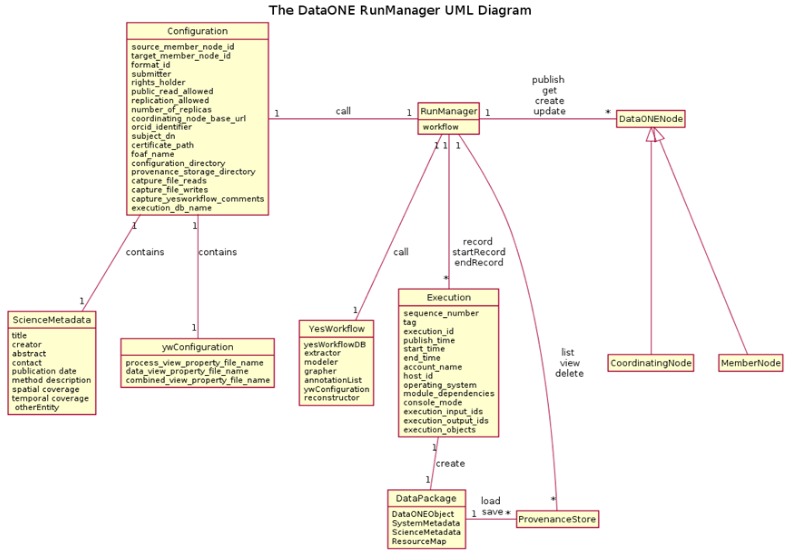
\includegraphics[height=11cm, width=13cm]{RunManagerUML}
%\caption{The DataONE RunManager UML Diagram }
%\label{fig:runManagerComponents}
%\end{figure}


\begin{figure}
\centering   
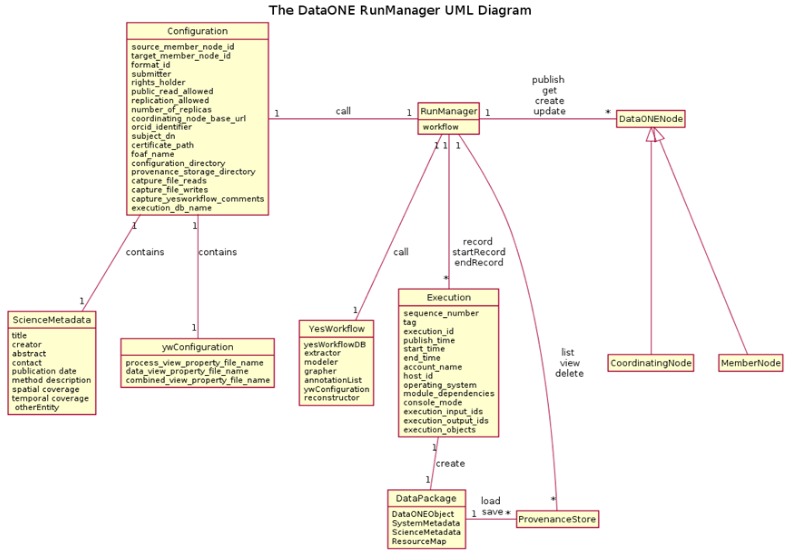
\includegraphics[width=1.2\textwidth]{RunManagerUML}
\caption{The principle classes with their attributes in matlab-dataone toolbox which is an implementation of the DataONE RunManager using Matlab and Java. In order to save space, the attributes for the \emph{CoordinatingNode}, \emph{MemberNode}, \emph{DataONEObject}, \emph{SystemMetadata} and \emph{ScienceMetadata} classes are not shown. }
\label{fig:runManagerComponents}
\end{figure}


The principal classes in the matlab-dataone toolbox and their composition are shown in Fig.~\ref{fig:runManagerComponents}. The labels on the arrows denote functions that can be used between different modules in the RunManager. Firstly, an Execution represents a script run, and contains some critical metadata needed to understand the execution environment, uniquely identify the run, categorize it, and know it's start and end times. Secondly, the Configuration class allows the scientist to configure the RunManager with properties such as the provenance information storage directory, DataONE target member node, DataONE coordinating node, and etc. The Configuration class contains an instance of ScienceMetadata and ywConfiguration. Thirdly, the DataONE DataPackage is used to store an RDF graph of the execution's members, and is serialized in the Open Archive Initiative's Object Re-use and Exchange (ORE) \cite{oaiore} format.  Input and output file objects are archived as DataONEObjects with system-level metadata that describe the objects. The RunManager assists in the preparation of science metadata, currently in the Ecological Metadata Language (EML) format, that describe the input and output science data objects associated with a script execution. Therefore, an DataPackage instance contains a list of instances of DataONEObjects, SystemMetadata, and ScienceMetadata. Lastly, the DataONENode class represents a DataONE Node and it is a superclass to the MemberNode and CoordinatingNode classes, providing shared DataONE API functions that can make provenance data available in the DataONE network. 

There are two ways to store the provenance data in the DataONE RunManager. At the current stage, data is stored in individual files on the local file systems for the matlab-dataone toolbox. But data is stored in a relational database for the recordr R package: there is only one copy for the input/output files. The copy of a file object is deleted when there is no reference pointing to it.

In the DataONE RunManager, prospective provenance is captured by the YesWorkflow (YW) \cite{yesworkflow} Java library which models conventional scripts and programs as scientific workflows. Instead of reimplementing code to be executed and managed by a workflow management system, a user embeds YW annotations within an existing script. These annotations declare how data will be used and derived by the script step by step. The YW library interprets the annotations and builds a graphical output that represents the script as a collection of entities, i.e., programs, workflows, ports, and channels which are mapped to the DataONE ProvONE model shown in \cite{provone-model}. 

DataONE has designed the ProvONE provenance data model to extend the W3C PROV data model \cite{prov} to express detail about the processes, ports, and data links common to scientific workflow systems. Both RunManager implementations in Matlab and R produce RDF provenance output adhering to the ProvONE data model so that the provenance information generated from different programming languages like R and Matlab can be shared in a common format.

The DataONE RunManager implementation automates the collection of retrospective provenance data. The automated collection is transparent to scientists and provides a medium-grained, rich account of the data dependencies.  More fine-grained automation approaches used in noWorkflow and RDataTracker result in voluminous provenance data. In our work, we currently focus on collecting file-level input and output data. 



\subsection{Overloading I/O Functions}

Our approach relies upon two basic techniques. First, we developed wrapper functions for commonly-used I/O functions in R and Matlab so that provenance information can be recorded as a script executes. The wrapper functions collect and store provenance information after calling the original I/O function. Second, during the initial installation of the R or Matlab libraries, the paths to these overloaded I/O functions are added to the function search path so that calls to original I/O functions are directed to the overloaded functions with the same function name in the library. 

\begin{algorithm}
\DontPrintSemicolon 
\KwIn{A number of input arguments $varargin=\{in_1, in_2, \ldots, in_n\}$}
\KwOut{A number of input arguments $varargout=\{out_1, out_2, \ldots, out_m\}$, two updated input/output Id lists, and an updated execution object map}
Get the RunManager instance\;
Remove the path to the overloaded functions from Matlab path\;
Call the native function with the same name\;
Add the path to the overloaded functions back to Matlab path\;
\eIf{the current file is a new data object}{
	Add this object to the execution objects map\;
}{
	Update the existing map entry with a new DataObject\;
}
Add the identifier of the current file to either the execution\_in\_ids or execution\_out\_ids set depending on the operation type \;  
\Return{$\{out_1, out_2, \ldots, out_m$, $execution\_input\_ids$, $execution\_output\_ids$, $execution\_objects$\}}\;

\caption{Steps for overloading a Matlab function in the Matlab DataONE Toolbox}
\label{algo:overloadFunctions}
\end{algorithm}

A set of functions to read and write data to files of different formats types are supported in the Matlab Dataone Toolbox and the recordr R package. The supported file formats include: MAT-files, text files, XML documents, Excel spreadsheets, scientific data in CDF, FITS, and HDF formats, audio/video files, graphical files, internet files, and DataONE get(), create(), update() API calls. 

The steps for overloading a Matlab function is shown in Algorithm 1. The method of overloading functions in R is different that in Matlab. When overloaded functions defined in the \emph{recordr} R package are to be used, a user only need to call \emph{library(recordr)} in the R console.  The R RunManager implementation overloads functions that read input and write output in order to capture the objects that are used and generated by the script execution. For instance, when a script reads in a CSV file, both RunManager implementations in Matlab and R can infer the triple $scriptExecution \rightarrow \emph{prov:used} \rightarrow .csv file$. The following PROV \cite{prov} provenance relationships are supported: prov:wasGeneratedBy, prov:used, prov:wasDerivedFrom, and prov:wasInformedBy.


%\subsection{ProvONE Data Model}

%\begin{figure}
%\centering
%\includegraphics[height=8.5cm, width=13.5cm]{provone-model}
%\caption{The DataONE ProvONE provenance data model will be used to describe the relationships between:
%Derived resources and the original resources used to create them,
%Data resources and the activities used to create them,
%Programs (e.g. software, scripts) that were implemented to create a data resource}
%\label{fig:provone-model}
%\end{figure}

%Both prospective provenance (i.e., the specification of the computation) and the retrospective provenance (i.e., the exact steps followed during the execution) contribute important information. DataONE has designed the ProvONE provenance data model to extend the W3C PROV data model to express detail about the processes, ports, and data links common to scientific workflow systems (see Figure~\ref{fig:provone-model}). Both RunManager implementations in Matlab and R produce RDF provenance output adhering to the ProvONE data model so that the provenance information generated from different programming languages like R and Matlab can be shared in a common format.



\subsection{Rendered at Web UI}


\section{Demo}   \label{demo}

Use Cases

1. Scientist Alice documents her script

2. Alice records the provenance of a script execution

3. Alice lists the given provenance information

4. Alice views a specific provenance

5. Alice publishes a provenance package to DataONE and shares the data package with other researchers


6. Scientist Bob views Alice's data package in web UI

7. Bob navigates between provenance relationships and downloads a whole data package

8. Interoperability between scripts in various programming lanaguages (R and Matlab)

Because the resource map is in RDF format which is independent of platformat 



\section{Future Work and Conclusions}   \label{future-work-conclusion}




\begin{thebibliography}{4}

\bibitem{noworkflow} Murta L, Braganholo V, Chirigati F, Koop D, Freire J. noWorkflow: Capturing and analyzing provenance of scripts. In: Lud{\"a}scher, B., Plate, B. (eds.) IPAW 2014. LNCS, vol. 8628,  pp. 71-83. Springer, Verlag. (2015)

\bibitem{yesworkflow} McPhillips T., Song T., Kolisnik T., Aulenbach S., Belhajjame K., Bocinsky R.K., Cao Y., Cheney J., Chirigati F., Dey S., Freire J., Jones C., Hanken J., Kintigh K.W., Kohler T.A., Koop D., Macklin J. A., Missier P., Schildhauer M., Schwalm C., Wei Y., Bieda M., and Ludascher B. YesWorkflow: A User-Oriented, Language-Independent Tool for Recovering Workflow Information from Scripts. International Journal for Digital Curation, vol. 10, 298--313. (2015)

\bibitem{oaiore} Open Archives Initiative Object Reuse and Exchange. \url{https://www.openarchives.org/ore/} (2008)

\bibitem{recordr} Slaughter P., Jones M., Jones C. NCEAS recordr: Provenance tracking for R. \url{https://github.com/NCEAS/recordr} (2016)

\bibitem{matlabdataone} Jones C., Cao Y., Slaughter P., Jones M. Matlab DataONE Toolbox. \url{https://github.com/DataONEorg/matlab-dataone} (2016)

\bibitem{prov} PROV-DM: The PROV Data Model. \url{http://www.w3.org/TR/prov-dm/} (2013)

\bibitem{sumatra} Davison A. Automated Capture of Experiment Context for Easier Reproducibility in Computational Research. Computing in Science \& Engineering, vol.14, no. 4, pp. 48--56. (2012)

\bibitem{rdatatracker} Lerner B., Boose E. RDataTracker: Collecting Provenance in an Interactive Scripting Environment. In: 6th USENIX Workshop on the Theory and Practice of Provenance, USENIX Association, Cologne. (2014)

\bibitem{provone-model} Walker L., Jones C., Jones M. The DataONE PROV Ontology and Model. \url{https://github.com/DataONEorg/sem-prov-design/blob/master/docs/PROV-annotation-model/PROVmodel.md} (2015)

\bibitem{cde} Guo P. and Engler D. CDE: Using System Call Interposition to Automatically Create Portable Software Packages. In: Proc. 2011 Usenix Annual Tech. Conf., Usenix Assoc. (2011)

\bibitem{sumatra-impl} Davison A.P., Mattioni M., Samarkanov D. and Tele\'{n}czuk B. Sumatra: A Toolkit for Reproducible Research. In: Implementing Reproducible Research, edited by V. Stodden, F. Leisch and R.D. Peng, Chapman \& Hall/CRC: Boca Raton, Florida., pp. 57-79. (2014)


%\bibitem{jour} Smith, T.F., Waterman, M.S.: Identification of Common Molecular
%Subsequences. J. Mol. Biol. 147, 195--197 (1981)

%\bibitem{lncschap} May, P., Ehrlich, H.C., Steinke, T.: ZIB Structure Prediction Pipeline:
%Composing a Complex Biological Workflow through Web Services. In: Nagel,
%W.E., Walter, W.V., Lehner, W. (eds.) Euro-Par 2006. LNCS, vol. 4128,
%pp. 1148--1158. Springer, Heidelberg (2006)

%\bibitem{book} Foster, I., Kesselman, C.: The Grid: Blueprint for a New Computing
%Infrastructure. Morgan Kaufmann, San Francisco (1999)

%\bibitem{proceeding1} Czajkowski, K., Fitzgerald, S., Foster, I., Kesselman, C.: Grid
%Information Services for Distributed Resource Sharing. In: 10th IEEE
%International Symposium on High Performance Distributed Computing, pp.
%181--184. IEEE Press, New York (2001)

%\bibitem{proceeding2} Foster, I., Kesselman, C., Nick, J., Tuecke, S.: The Physiology of the
%Grid: an Open Grid Services Architecture for Distributed Systems
%Integration. Technical report, Global Grid Forum (2002)

%\bibitem{url} National Center for Biotechnology Information, \url{http://www.ncbi.nlm.nih.gov}

\end{thebibliography}


%\section*{Appendix: Springer-Author Discount}


%\section{Checklist of Items to be Sent to Volume Editors}
%Here is a checklist of everything the volume editor requires from you:


%\begin{itemize}
%\settowidth{\leftmargin}{{\Large$\square$}}\advance\leftmargin\labelsep
%\itemsep8pt\relax
%\renewcommand\labelitemi{{\lower1.5pt\hbox{\Large$\square$}}}

%\item The final \LaTeX{} source files
%\item A final PDF file
%\item A copyright form, signed by one author on behalf of all of the
%authors of the paper.
%\item A readme giving the name and email address of the
%corresponding author.
%\end{itemize}

\end{document}
